\chapter{Solution Overview}
Our work on the project could be divided into 4 different aspects we focused on. The task required us to create our own dataset for neural network training, as well as to devise an algorithm calculating objects' bounding boxes. The program had to be then connected to the RGBD cameras and made into a user-friendly application. The following flowchart illustrates the working principle of the program:

\begin{figure}[ht]
    \centering
    \includesvg[scale=0.4]{img/app-flowchart.svg}
    \caption{Flowchart showing the program's operating principle.}
    \label{fig:app-flowchart}
\end{figure}

\section{Dataset preparation}
After considering the size of the photo box and the availability of certain everyday objects, we chose 7 different classes:
\begin{itemize}[noitemsep,topsep=0pt,parsep=0pt,partopsep=0pt]
    \item mug
    \item box
    \item wine glass
    \item bowl
    \item shoe
    \item cap
    \item lamp
\end{itemize}
Our initial plans were to also include a \textit{bottle} class, however after encountering several problems, mainly concerning the way the light rays passed through the bottles, we were forced to narrow it down.

\subsection{Obtaining photo data}
To obtain RGB and depth image data we used Intel's \textit{RealSense Viewer} application, which is a part of Intel® RealSense™ SDK 2.0 \cite{realsense-sdk}. We recorded short sequences and saved them as .bag files, from which we later extracted the RGB image and depth data in form of a point cloud.

\begin{figure}[ht]
    \centering
    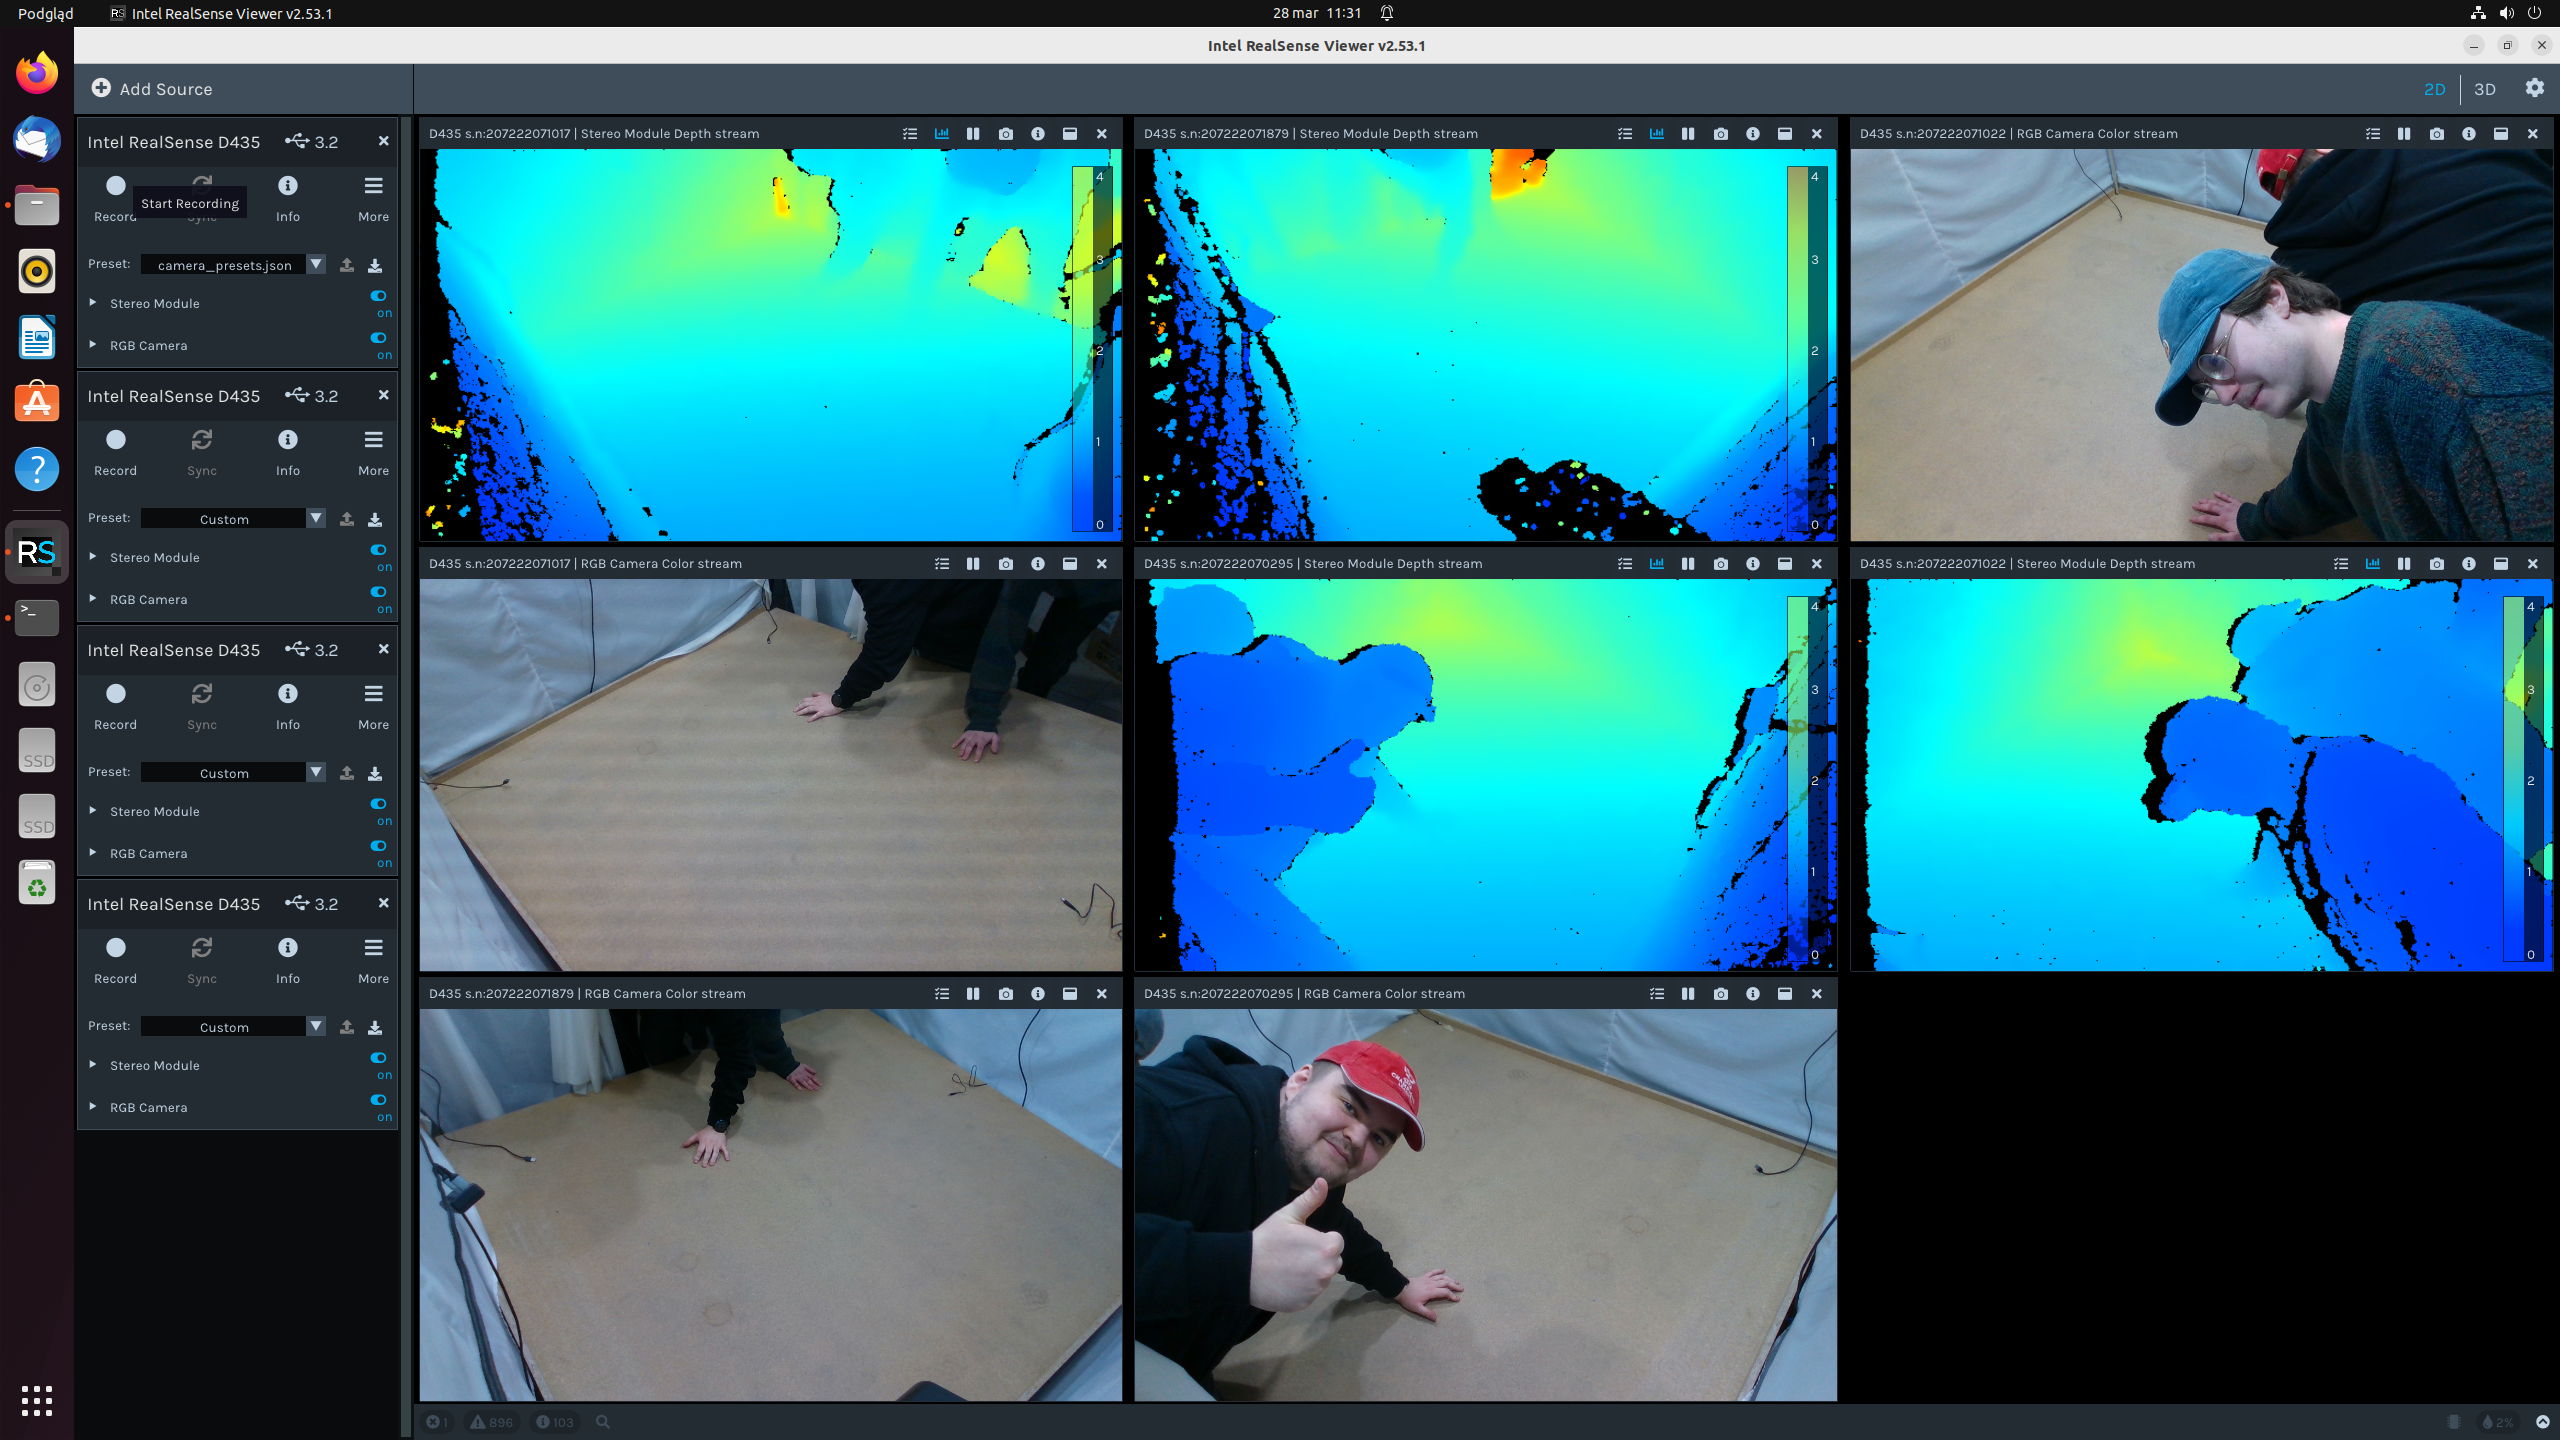
\includegraphics[width=0.75\textwidth]{img/viewer-screenshot.png}
    \caption{Intel's RealSense Viewer window showing capturing data from the cameras.}
    \label{fig:realsense-viewer}
\end{figure}

Preparing the data in the lab took about 15 hours. Overall we captured close to 900 images, with over 5000 single object occurrences. 

\subsection{Labelling photos}
For labelling the instances we used a free online tool \textit{labelbox.com} \cite{labelbox}. It enabled us to work simultaneously as a group and provided an easy way to apply masks to our images.

\begin{figure}[ht]
    \centering
    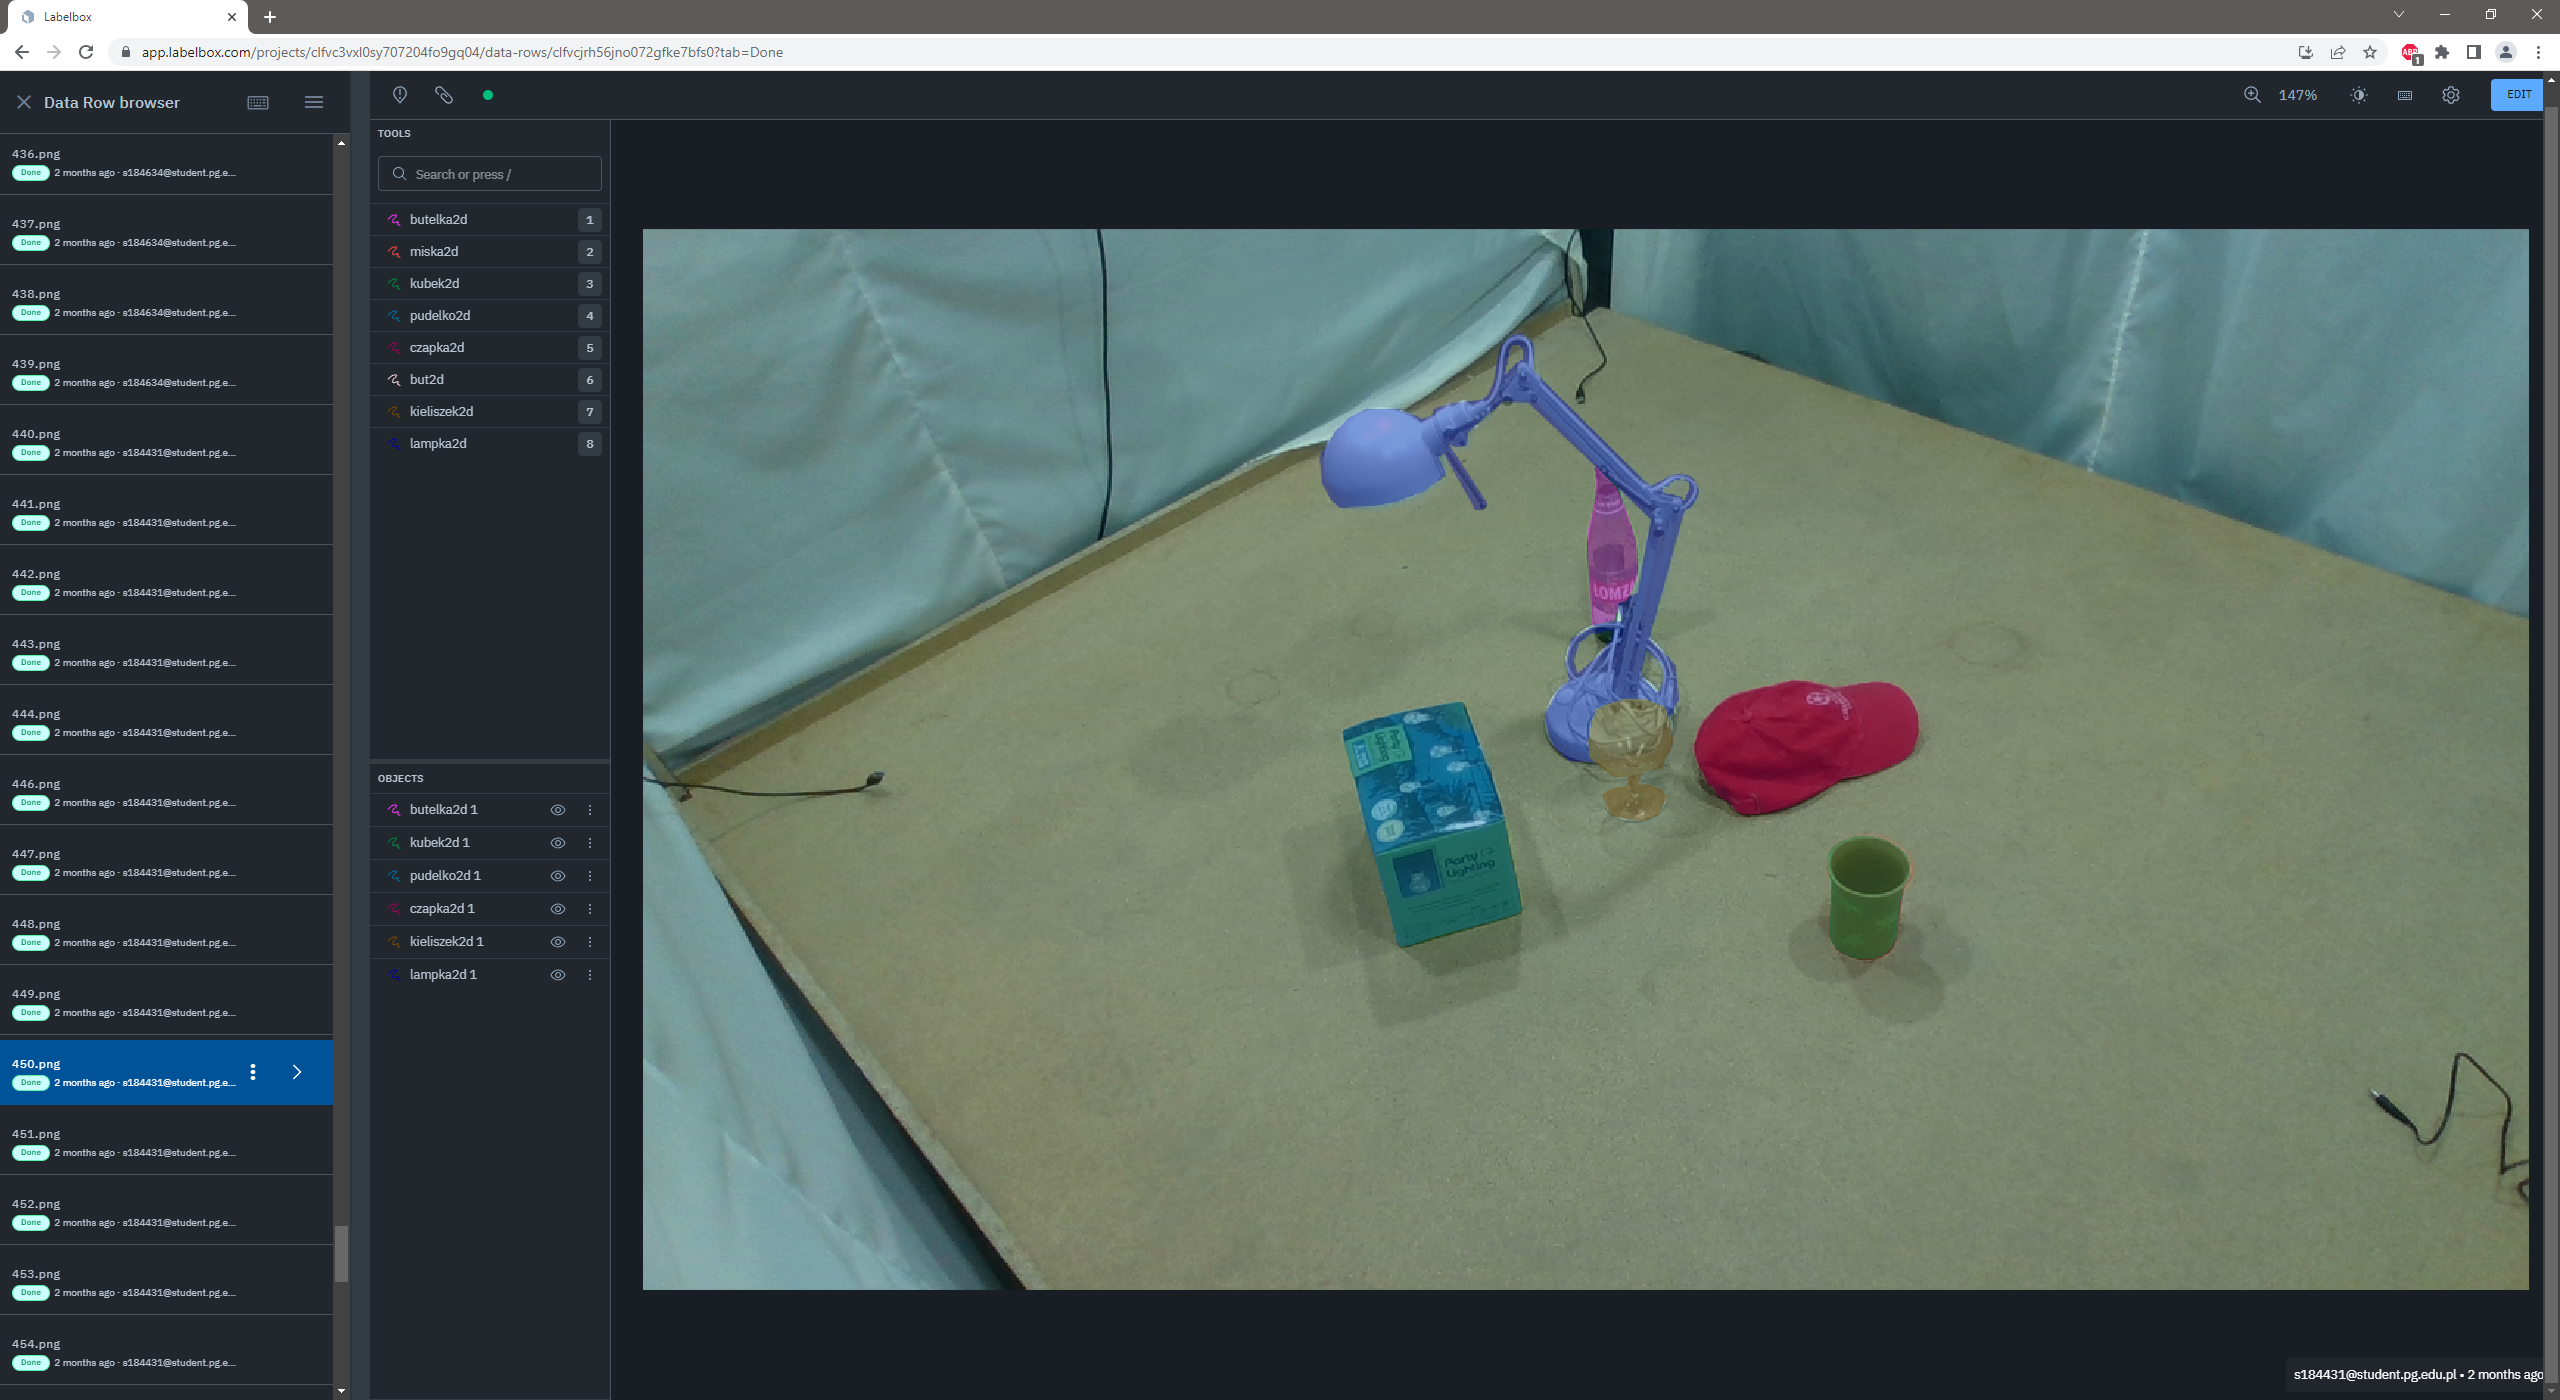
\includegraphics[width=0.8\textwidth]{img/labelbox-screenshot.png}
    \caption{One of the images from the dataset annotated in labelbox.}
    \label{fig:labelbox-window}
\end{figure}

Annotating, reviewing and reworking the images took 52 hours in total and was on of the most time-consuming tasks our team had to deal with.

\section{Segmentation algorithm}
Our Instance

\subsection{MaskRCNN for object segmentation in 2D}
We decided to use Mask R-CNN because it is a state-of-the-art Deep Convolutional Neural Network regarding image segmentation \cite{he2018mask, matterport_maskrcnn_2017}. This Neural Network detects objects in an image and generates a high-quality segmentation mask for each instance. It provides the vector of three essential factors for each object: instance mask, bounding box and label. Each of those elements is used in the following stages of image analysis (\cref{fig:app-flowchart}).

In our solution, the network got fine-tuned \cite{shinya2019understanding} on the dataset we made. The version used is Mask R-CNN v2 with a ResNet-50-FPN backbone \cite{li2021benchmarking}.

\subsection{Integration with the RGBD cameras}
We used the pyrealsense2 \cite{pyrealsense2-doc} library to get aligned RGB and depth frames from the cameras, and also to filter the depth image with temporal and spatial filtering. The RGB image is used as the input to MaskRCNN and the output masks are applied to the filtered depth image. This allows us to retrieve separate depth images of all the detected objects in the scene. These images are then used to create separate point clouds and draw bounding boxes around them using Open3D \cite{Zhou2018open3d}. The bounding boxes’ coordinates are extracted and used to project them onto the original RGB image.

\subsection{3D bounding boxes}
After familiarising ourselves with the concept of 3D bounding boxes (\textit{3DBB}) and the already existing methods of determining their placements \cite{MousavianAFK16}, we have devised our own 3DBB creating method relying on the functionalities of Open3D python library \cite{Zhou2018open3d} and processing of the point cloud. The first stage consists of extracting a part of the point cloud with our analysed object, based on its mask (\cref{fig:3dbb-mask}). To do that, we use Open3D, creating the object's bounding box (\cref{fig:pcloud-cutout}).

\begin{figure}[ht]
    \centering
    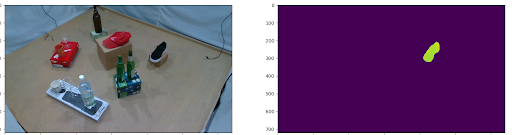
\includegraphics[width=0.8\textwidth]{img/mask.png}
    \caption{An example showing the RGB image and the mask of an object.}
    \label{fig:3dbb-mask}
\end{figure}

\begin{figure}[ht]
    \centering
    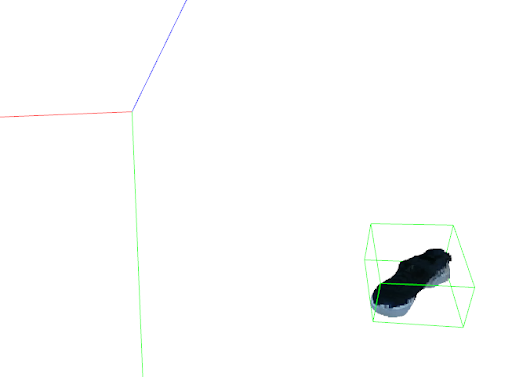
\includegraphics[width=0.4\textwidth]{img/pcloud-cutout.png}
    \caption{Fragment of the point cloud containing the previously shown object, with RGB image applied and a visible bounding box.}
    \label{fig:pcloud-cutout}
\end{figure}

After that, by getting the positions of 3DBB's vertices in the 3D space, the vertices' coordinates are transformed and properly placed on the 2D image using the OpenCV python library \cite{opencv_library}. The points are then connected by lines, comprising a 3D bounding box projected onto a two-dimensional plane (\cref{fig:pbbox-example}.

\begin{figure}[ht]
    \centering
    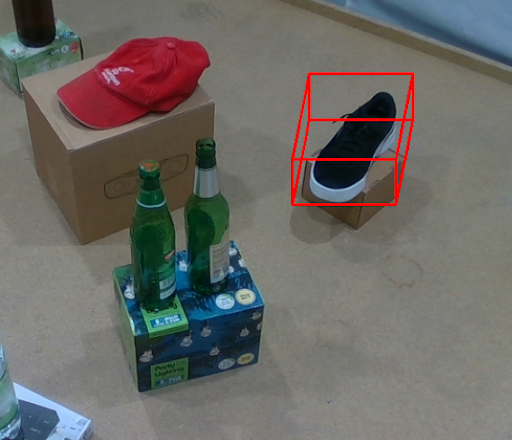
\includegraphics[width=0.4\textwidth]{img/bbox-example.png}
    \caption{A fragment of an RGB image showing the projected bounding box for an object.}
    \label{fig:pbbox-example}
\end{figure}

A key piece of information used while projecting the 3DBBs is the depth data, which has to be taken into account with the loss of the \textit{Z} dimension. It also allows us to determine the proportions of the boxes' edges to one another, which aids in the inspection of the projected points and automatic correction of their locations if any errors are found. The position of the 3DBB is checked in relation to the position of the object's mask, and in case of too big of a deviation, the bounding box's dimensions are corrected. 

Overall, we introduced a significant amount of parameters, which values were determined by trial and error, as well as variables which helped us control the correctness of the final coordinates of points on the 2D plane to properly replicate a 3D bounding box in a known environment and under known conditions. Of course, our approach is not perfect, and there are more accurate methods in existence. However, it does allow us to reconstruct an object's bounding box to a sufficient degree without using neural networks.

